\documentclass{article}

\usepackage{amsmath}
\usepackage{amssymb}
\usepackage{bm}
\usepackage{color}
\usepackage{CJKutf8}
\usepackage{color}
\usepackage{enumitem}
\usepackage{graphicx}
\usepackage{listings}
\usepackage{mathdots}
\usepackage{tikz}
\usepackage{wasysym}
\usepackage{xcolor}

\usetikzlibrary{shapes,arrows}

\allowdisplaybreaks

\begin{document}
\begin{CJK*}{UTF8}{gbsn}

\title{homework 2}
\author{计算机1202 张艺瀚}
\maketitle

给定\verb|0-1|背包问题,\verb|n=5|, \verb|c=50|, \verb|v=[12, 44, 46, 30, 50]|, \verb|w=[5, 25, 27, 15, 30]|。 \\
\begin{enumerate}
\item 采用回溯法求解该问题,分别用表格形式和解空间树形式跟踪算法执行过程。
\item 采用分支限界法求解该问题,跟踪算法执行过程,给出解空间树和活结点优先队列的更新过程。
\end{enumerate}

\section{backtrack}

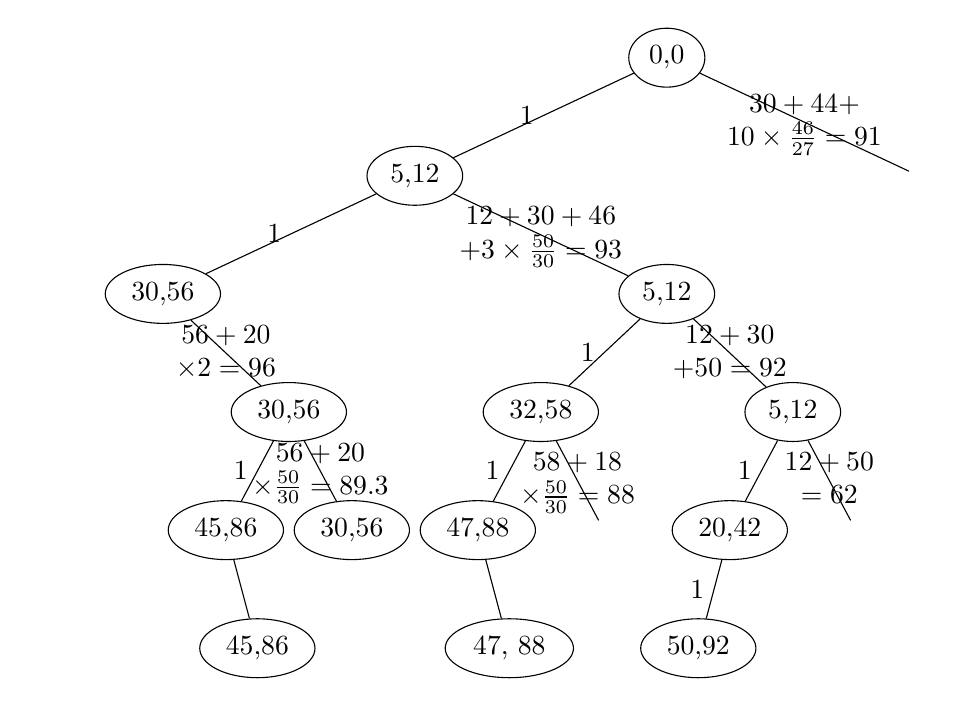
\begin{tikzpicture}
\tikzstyle{level 1} = [sibling distance = 64mm]
\tikzstyle{level 2} = [sibling distance = 64mm]
\tikzstyle{level 3} = [sibling distance = 32mm]
\tikzstyle{level 4} = [sibling distance = 16mm]
\tikzstyle{level 5} = [sibling distance = 8mm]
\tikzstyle{level 6} = [sibling distance = 4mm]
\node[ellipse, draw] {0,0}
	child {node[ellipse, draw] {5,12}
		child {node[ellipse, draw] {30,56}
			child {node {} edge from parent[draw = none]}
			child {node[ellipse, draw] {30,56}
				child {node[ellipse, draw] {45,86}
					child {node {} edge from parent[draw = none]}
					child {node[ellipse, draw] {45,86}}
					edge from parent[left]
						node {1}
				}
				child {node[ellipse, draw] {30,56}
					edge from parent
						node {
							\begin{tabular}{c}
								$56+20$ \\
								$\times\frac{50}{30}=89.3$
							\end{tabular}
						}
				}
				edge from parent
					node {
						\begin{tabular}{c}
							$56+20$ \\
							$\times 2=96$
						\end{tabular}
					}
			}
			edge from parent[left]
				node {1}
		}
		child {node[ellipse, draw] {5,12}
			child {node[ellipse, draw] {32,58}
				child {node[ellipse, draw] {47,88}
					child {node {} edge from parent[draw = none]}
					child {node[ellipse, draw] {47, 88}}
					edge from parent[left]
						node {1}
				}
				child {node {}
					edge from parent
						node {
							\begin{tabular}{c}
								$58+18$ \\
								$\times\frac{50}{30}=88$
							\end{tabular}
						}
				}
				edge from parent[left]
					node {1}
			}
			child {node[ellipse, draw] {5,12}
				child {node[ellipse, draw] {20,42}
					child {node[ellipse, draw] {50,92}
						edge from parent[left]
							node {1}
					}
					child {node {} edge from parent[draw = none]}
					edge from parent[left]
						node {1}
				}
				child {node {}
					edge from parent
						node {
							\begin{tabular}{c}
								$12+50$ \\
								$=62$
							\end{tabular}
						}
				}
				edge from parent
					node {
						\begin{tabular}{c}
							$12+30$ \\
							$+50=92$
						\end{tabular}
					}
			}
			edge from parent
				node {
					\begin{tabular}{c}
						$12+30+46$ \\
						$+3\times\frac{50}{30}=93$
					\end{tabular}
				}
		}
		edge from parent[left]
			node {1}
	}
	child {node {}
		edge from parent
			node {
				\begin{tabular}{c}
					$30+44+$ \\
					$10\times\frac{46}{27}=91$
				\end{tabular}
			}
	};
\end{tikzpicture}

\begin{center}
\begin{tabular}{|l|l|l|l|l|l|l|l|l|}
\hline
$i$	&$x_1$			&$x_2$			&$x_3$			&$x_4$			&$x_5$			&$cw$		&$cp$		&$bestp$\\ \hline
1	&0				&0				&0				&0				&0				&0			&0			&0		\\ \hline
1	&\underline{1}	&0				&0				&0				&0				&5			&12			&0		\\ \hline
2	&\underline{1}	&\underline{1}	&0				&0				&0				&30			&56			&0		\\ \hline
3	&\underline{1}	&\underline{1}	&\underline{0}	&0				&0				&30			&56			&0		\\ \hline
4	&\underline{1}	&\underline{1}	&\underline{0}	&\underline{1}	&0				&45			&86			&0		\\ \hline
5	&\underline{1}	&\underline{1}	&\underline{0}	&\underline{1}	&\underline{0}	&45			&86			&0		\\ \hline
6	&\underline{1}	&\underline{1}	&\underline{0}	&\underline{1}	&\underline{0}	&45			&86			&86		\\ \hline
4	&\underline{1}	&\underline{1}	&\underline{0}	&\underline{0}	&0				&30			&56			&86		\\ \hline
2	&\underline{1}	&\underline{0}	&0				&0				&0				&5			&12			&86		\\ \hline
3	&\underline{1}	&\underline{0}	&\underline{1}	&0				&0				&32			&58			&86		\\ \hline
4	&\underline{1}	&\underline{0}	&\underline{1}	&\underline{1}	&0				&47			&88			&86		\\ \hline
5	&\underline{1}	&\underline{0}	&\underline{1}	&\underline{1}	&\underline{0}	&47			&88			&86		\\ \hline
6	&\underline{1}	&\underline{0}	&\underline{1}	&\underline{1}	&\underline{0}	&47			&88			&88		\\ \hline
3	&\underline{1}	&\underline{0}	&\underline{0}	&0				&0				&5			&12			&88		\\ \hline
4	&\underline{1}	&\underline{0}	&\underline{0}	&\underline{1}	&0				&20			&42			&88		\\ \hline
5	&\underline{1}	&\underline{0}	&\underline{0}	&\underline{1}	&\underline{1}	&50			&92			&88		\\ \hline
6	&\underline{1}	&\underline{0}	&\underline{0}	&\underline{1}	&\underline{1}	&50			&92			&92		\\ \hline
\end{tabular}
\end{center}

\section{branch and bound}

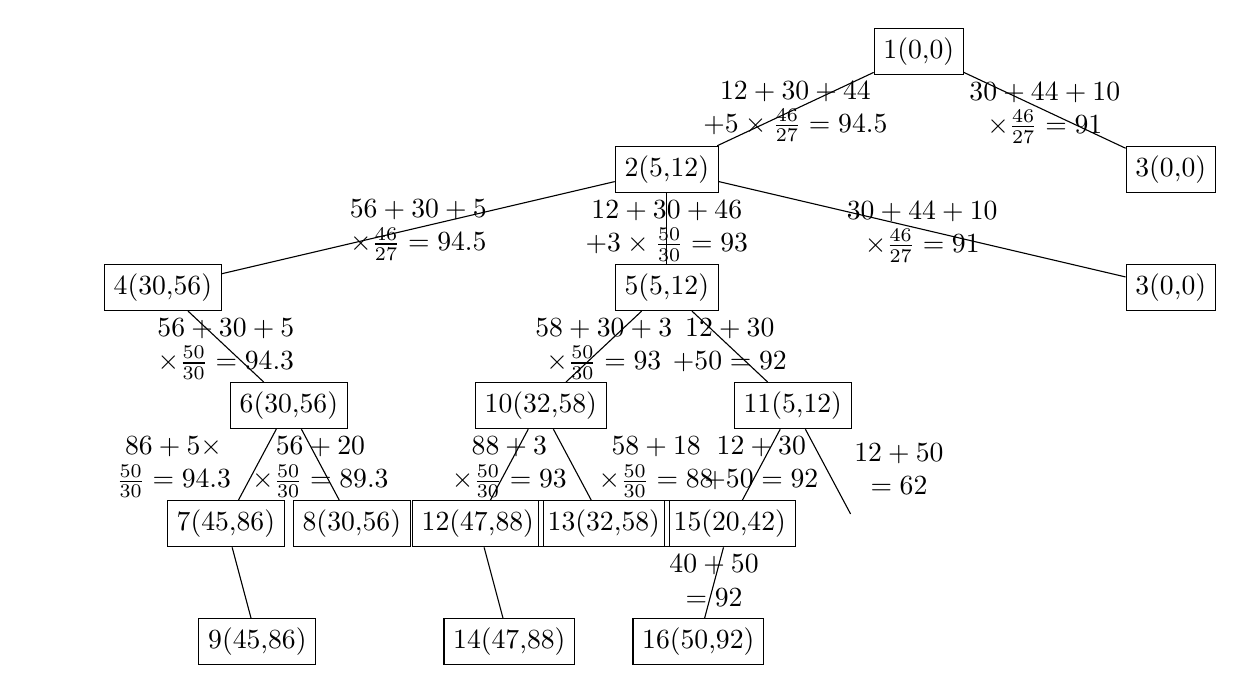
\begin{tikzpicture}
\tikzstyle{level 1} = [sibling distance = 64mm]
\tikzstyle{level 2} = [sibling distance = 64mm]
\tikzstyle{level 3} = [sibling distance = 32mm]
\tikzstyle{level 4} = [sibling distance = 16mm]
\tikzstyle{level 5} = [sibling distance = 8mm]
\tikzstyle{level 6} = [sibling distance = 4mm]
\node[rectangle, draw] {1(0,0)}
	child {node[rectangle, draw] {2(5,12)}
		child {node[rectangle, draw] {4(30,56)}
			child {node {} edge from parent[draw = none]}
			child {node[rectangle, draw] {6(30,56)}
				child {node[rectangle, draw] {7(45,86)}
					child {node {} edge from parent[draw = none]}
					child {node[rectangle, draw] {9(45,86)}}
					edge from parent[left]
						node {
							\begin{tabular}{c}
								$86+5\times$ \\
								$\frac{50}{30}=94.3$
							\end{tabular}
						}
				}
				child {node[rectangle, draw] {8(30,56)}
					edge from parent
						node {
							\begin{tabular}{c}
								$56+20$ \\
								$\times \frac{50}{30}=89.3$
							\end{tabular}
						}
				}
				edge from parent
					node {
						\begin{tabular}{c}
							$56+30+5$ \\
							$\times \frac{50}{30}=94.3$
						\end{tabular}
					}
			}
			edge from parent
				node {
					\begin{tabular}{c}
						$56+30+5$ \\
						$\times \frac{46}{27}=94.5$
					\end{tabular}
				}
		}
		child {node[rectangle, draw] {5(5,12)}
			child {node[rectangle, draw] {10(32,58)}
				child {node[rectangle, draw] {12(47,88)}
					child {node {} edge from parent[draw = none]}
					child {node[rectangle, draw] {14(47,88)}}
					edge from parent
						node {
							\begin{tabular}{c}
								$88+3$ \\
								$\times \frac{50}{30}=93$
							\end{tabular}
						}
				}
				child {node[rectangle, draw] {13(32,58)}
					edge from parent[right]
						node {
							\begin{tabular}{c}
								$58+18$ \\
								$\times \frac{50}{30}=88$
							\end{tabular}
						}
				}
				edge from parent
					node {
						\begin{tabular}{c}
							$58+30+3$ \\
							$\times \frac{50}{30}=93$
						\end{tabular}
					}
			}
			child {node[rectangle, draw] {11(5,12)}
				child {node[rectangle, draw] {15(20,42)}
					child {node[rectangle, draw] {16(50,92)}
						edge from parent
							node {
								\begin{tabular}{c}
									$40+50$ \\
									$=92$
								\end{tabular}
							}
					}
					child {node {} edge from parent[draw = none]}
					edge from parent
						node {
							\begin{tabular}{c}
								$12+30$ \\
								$+50=92$
							\end{tabular}
						}
				}
				child {node {}
					edge from parent[right]
						node {
							\begin{tabular}{c}
								$12+50$ \\
								$=62$
							\end{tabular}
						}
				}
				edge from parent
					node {
						\begin{tabular}{c}
							$12+30$ \\
							$+50=92$
						\end{tabular}
					}
			}
			edge from parent
				node {
					\begin{tabular}{c}
						$12+30+46$ \\
						$+3 \times \frac{50}{30}=93$
					\end{tabular}
				}
		}
		child {node[rectangle, draw] {3(0,0)}
			edge from parent
				node {
					\begin{tabular}{c}
						$30+44+10$ \\
						$\times \frac{46}{27}=91$
					\end{tabular}
				}
		}
		edge from parent
			node {
				\begin{tabular}{c}
					$12+30+44$ \\
					$+5 \times \frac{46}{27} = 94.5$
				\end{tabular}
			}
	}
	child {node[rectangle, draw] {3(0,0)}
		edge from parent
			node {
				\begin{tabular}{c}
					$30+44+10$ \\
					$\times \frac{46}{27}=91$
				\end{tabular}
			}
	};
\end{tikzpicture}

\newpage
\verb|priority queue|

\begin{center}
\begin{tabular}{|l|l|l|l|l|l|}
\hline
1(0)	&		&		&		&		&		\\ \hline
2(94.5)	&3(91)	&		&		&		&		\\ \hline
4(94.5)	&5(93)	&3(91)	&		&		&		\\ \hline
6(94.3)	&5(93)	&3(91)	&		&		&		\\ \hline
7(94.3)	&5(93)	&3(91)	&8(89.3)&		&		\\ \hline
5(93)	&3(91)	&8(89.3)&9(86)	&		&		\\ \hline
10(93)	&11(92)	&3(91)	&8(89.3)&9(86)	&		\\ \hline
12(93)	&11(92)	&3(91)	&8(89.3)&13(88)	&9(86)	\\ \hline
11(92)	&3(91)	&8(89.3)&13(88)	&14(88)	&9(86)	\\ \hline
15(92)	&3(91)	&8(89.3)&13(88)	&14(88)	&9(86)	\\ \hline
16(92)	&3(91)	&8(89.3)&13(88)	&14(88)	&9(86)	\\ \hline
\end{tabular}
\end{center}

\end{CJK*}
\end{document}
